In this chapter we report a formal analysis of the system performed with the specification language Alloy, along with the output of Alloy Analyzer, in order to check the correctness and coherence of the logical components of the system.

\subsection{Signatures}
In this section, we list the signatures used in the formal analysis. Note that the description of the various components includes only the elements that are at interest in the formal analysis.

\begin{minted}{alloy}
open util/integer
open util/boolean

sig Email,Name {}
sig EducatorEmail,EducatorName {}

sig Badge{
    tournament: one Tournament
}

sig Student{
    name: one Name,
    email: one Email,
    //The set of earned badges
    var badges: set Badge
}

enum GroupStatus{
    //The group has not been created yet
    GroupNotCreatedYet,
    //The group has been created but it has not been accepted yet
    GroupPending,
    //The group has been accepted and its members can now solve the battle
    GroupValid,
    //The group has not been accepted
    GroupRejected
}

sig Group{
    var students: set Student,
    var status: one GroupStatus
}

sig Educator{
    name: one EducatorName,
    email: one EducatorEmail
}

enum TournamentStatus{
    //The tournament has not been created yet
    TournamentNotCreatedYet,
    //The tournament has been created and it accepts Registrations
    TournamentRegistration,
    //The tournament has started,
    //students can solve battles within the tournament
    TournamentStarted,
    //The tournament has been closed
    TournamentClosed
}

sig Tournament{
    creator: one Educator,
    var status: one TournamentStatus,
    //The set of students subscripted to the tournament
    var students: set Student
}

enum BattleStatus{
    //The battle has not been created yet
    BattleNotCreatedYet,
    //The battle has been created and it accepts Registrations
    BattleRegistration,
    //The battle has started, groups can submit their solutions
    BattleStarted,
    //The solutions are manually evaluated by the educator
    BattleConsolidation,
    //The battle has been closed
    BattleClosed
}

sig Battle{
    creator: one Educator,
    tournament: one Tournament,
    //Minimum and maximum students per group
    minStudentPerGroup: one Int,
    maxStudentPerGroup: one Int,
    //Groups partecipating to the battle
    var groups: set Group,
    //Groups enlisted for the battle but not yet confirmed
    var pendingGroups: set Group,
    var status: one BattleStatus,
    //True if the educator manually evaluates the solutions
    consolidationPhase: one Bool
}
\end{minted}

\subsection{Time-independent facts}
Alloy facts allow the model to behave coherently with the real world. Facts can depend or not on the time evolution of the system: in this section, we report the static, time-independent facts, while the next sections will analyze time-dependent variables and their interactions.

\begin{minted}{alloy}
//All Emails correspond to at least a Student
fact NoUnusedEmails{
    no e:Email | (no s:Student | s.email = e)
}
//All Names correspond to at least a Student
fact NoUnusedNames{
    no n:Name | (no s:Student | s.name = n)
}
//All EducatorEmails correspond to at least an Educator
fact NoUnusedEducatorEmails{
    no e:EducatorEmail | (no ed:Educator | ed.email = e)
}
//All EducatorNames correspond to at least an Educator
fact NoUnusedEducatorNames{
    no n:EducatorName | (no ed:Educator | ed.name = n)
}

//All the students have unique Emails
fact UniqueEmailForStudents{
    no disj s1,s2:Student | s1.email = s2.email
}
//All the educators have unique Emails
fact UniqueEmailForEducators{
    no disj e1,e2:Educator | e1.email = e2.email
}

//The minimum and maximum number of students per group must be coherent
fact CoherentGroupConstraintsInBattle{
    all b:Battle | b.minStudentPerGroup > 0
    and (b.maxStudentPerGroup >= b.minStudentPerGroup)
}
\end{minted}

\subsection{Tournaments}
The following facts model the correct evolution of the state of each tournament, along with some considerations on the battles contained in the tournament and the students subscribed to it.

\begin{minted}{alloy}
//Every Tournament is initially not created
fact BeginningNotCreatedYet{
    all t:Tournament | always(
    (t.status = TournamentNotCreatedYet implies
    historically t.status = TournamentNotCreatedYet) and
    (t.status != TournamentNotCreatedYet implies
    once t.status = TournamentNotCreatedYet))
}

//Transition predicates
pred TournamentNotCreatedYetToRegistration[t:Tournament]{
    t.status = TournamentNotCreatedYet
    t.status' = TournamentRegistration
}
pred TournamentRegistrationToStarted[t:Tournament]{
    t.status = TournamentRegistration
    t.status' = TournamentStarted
}
pred TournamentStartedToClosed[t:Tournament]{
    t.status = TournamentStarted
    t.status' = TournamentClosed
}

//All the changes in the tournament status follow the defined transitions
fact TransitionsFact{
    all t:Tournament | always( 
    t.status'=t.status or
    TournamentNotCreatedYetToRegistration[t] or
    TournamentRegistrationToStarted[t] or
    TournamentStartedToClosed[t])
}

//For the tournament to close, all the battles have to be closed
fact TournamentsClose{
    all t: Tournament | always(
        t.TournamentStartedToClosed implies (
            all b:Battle | b.tournament = t implies b.status' = BattleClosed
        )
    )
}

//All the tournaments eventally close
fact TournamentsClose{
    all t: Tournament | eventually t.status = TournamentClosed
}

//The students can subscribe only in the Registration phase
fact RegistrationsInTournament{
    all t:Tournament | always(
    (t.status = TournamentNotCreatedYet implies #t.students = 0 ) and
    (t.students' != t.students implies t.status' = TournamentRegistration))
}
\end{minted}

\subsection{Student groups}
The following facts model the correct formation of teams within students that want to solve together a specific battle, along with the evolution of the teams' status.

\begin{minted}{alloy}
//The groups start from an initial state
fact GroupInitialState{
    all g:Group | once( g.status = GroupNotCreatedYet )
}

//Group state transitions
pred GroupNotCreatedYetToPending[g:Group]{
    g.status = GroupNotCreatedYet
    g.status' = GroupPending
}
pred GroupPendingToValid[g:Group]{
    g.status = GroupPending
    g.status' = GroupValid
}
pred GroupPendingToRejected[g:Group]{
    g.status = GroupPending
    g.status' = GroupRejected
}

//The group status must follow the possible transitions
fact GroupTransitions{
    all g:Group | always(
        g.status = g.status' or
        GroupNotCreatedYetToPending[g] or
        GroupPendingToValid[g] or
        GroupPendingToRejected[g]
    )
}

//A group must be initially created by at least one student
fact GroupsCreatedBySomeStudents{
    all g:Group | always(
        GroupNotCreatedYetToPending[g] implies #g.students' > 0
    )
}

//Students can join a group only when it is "pending"
fact StudentsJoinGroupsWhenCreated{
    all g:Group | always(
        (g.status = GroupNotCreatedYet implies #g.students = 0) and
        (g.students' != g.students implies g.status' = GroupPending)
    )
}

//A group is pending only if it is enlisted in a battle
fact PendingIfInBattlePendingGroups{
    all g:Group | always(
        g.status = GroupPending iff one b:Battle | g in b.pendingGroups
    )
}

//A group is valid only if it is accepted in a battle
fact ValidIfInBattleValidGroups{
    all g:Group | always(
        g.status = GroupValid iff one b:Battle | g in b.groups
    )
}

//No unused groups
fact NoUnusedGroups{
    all g:Group | eventually (g.status = GroupValid or g.status = GroupRejected)
}

//A group exists in the context of just one battle
fact NoGroupsInMultipleBattles{
    all g:Group | 
    (no disj b1,b2:Battle |
        once (g in b1.pendingGroups) and
        once (g in b2.pendingGroups))
}
\end{minted}

\subsection{Code Kata Battles}
These facts model the correct evolution in time of each battle, keeping into consideration all the context parameters such as the tournament they are in and the students that want to partecipate.

\begin{minted}{alloy}
//The battles start from an initial state
fact BattleInitialState{
    all b:Battle | once( b.status = BattleNotCreatedYet )
}

//Battle state transitions
pred BattleNotCreatedYetToRegistration[b:Battle]{
    b.status = BattleNotCreatedYet
    b.status' = BattleRegistration
}
pred BattleRegistrationToStarted[b:Battle]{
    b.status = BattleRegistration
    b.status' = BattleStarted
}
pred BattleStartedToConsolidation[b:Battle]{
    b.status = BattleStarted
    b.status' = BattleConsolidation
}
pred BattleStartedToClosed[b:Battle]{
    b.status = BattleStarted
    b.status' = BattleClosed
}
pred BattleConsolidationToClosed[b:Battle]{
    b.status = BattleConsolidation
    b.status' = BattleClosed
}

//The battle status must follow the possible transitions
fact BattleTransitions{
    all b:Battle | always(
        b.status' = b.status or
        BattleNotCreatedYetToRegistration[b] or
        BattleRegistrationToStarted[b] or
        BattleStartedToConsolidation[b] or
        BattleStartedToClosed[b] or
        BattleConsolidationToClosed[b]
    )
}

//The consolidation phase happens only when necessary
fact ConsolidationPhaseWhenNecessary{
    all b:Battle | always(
        BattleStartedToConsolidation[b] implies b.consolidationPhase.isTrue and
        BattleStartedToClosed[b] implies b.consolidationPhase.isFalse
    )
}

//The battle can be created only when the tournament has started
fact BattleInStartedTournament{
    all b:Battle | always(
        BattleNotCreatedYetToRegistration[b] implies
        b.tournament.status' = TournamentStarted)
}

//Students can register to a battle only if they are registered
//to the tournament
fact AllGroupStudentsInTournament{
    all b:Battle | always(
        no s:Student | s not in b.tournament.students and
        s in b.(groups + pendingGroups).students
    )
}

//Student cannot register in two groups for the same battle
fact NoStudentInTwoGroupsSameBattle{
    all b:Battle | always(
        no disj g1,g2:b.(groups + pendingGroups) | (
            some s:Student | (
                (s in g1.students) and (s in g2.students) )))
}
\end{minted}

\subsection{Interaction between Groups and Battles}
Since the interaction between Groups and Battles is crucial for the correctness of the model, this dedicated paragraph lists all the facts necessary for a correct time evolution of these entities.

\begin{minted}{alloy}
//Groups can register only during the Battle Registration phase
fact GroupsRegistrationDuringRegistrationPhase{
    all b:Battle | always(
        (b.status = BattleNotCreatedYet implies
        #b.groups = 0 and #b.pendingGroups = 0) and
        (b.status = BattleRegistration implies #b.groups = 0) and
        ((b.status = BattleStarted or b.status = BattleConsolidation or
        b.status = BattleClosed) implies
        #b.pendingGroups = 0 and b.groups = b.groups'))
}

//Groups can partecipate to the battle only if they are valid
fact OnlyValidGroupsPartecipate{
    all b:Battle | always(
        all g:b.groups | g.status = GroupValid
    )
}

//Groups get accepted only if they have the correct number of students
fact OnlyGroupsWithCorrectStudentsGetAccepted{
    all b:Battle | always(
        all g:b.groups | (
            #g.students >= b.minStudentPerGroup and
            #g.students <= b.maxStudentPerGroup and 
            once g in b.pendingGroups))
}

//Groups pending cannot invite more than maxStudentPerGroup students
fact NoMoreThanMaxStudentsPerGroup{
    all b:Battle | always(
        all g:b.pendingGroups | #g.students <= b.maxStudentPerGroup
    )
}

//Groups get rejected only if they have an incorrect number of students
//when the battle starts
fact RejectedGroupsHaveIncorrectStudents{
    all g:Group | always(
        GroupPendingToRejected[g] iff (
            one b:Battle | ( BattleRegistrationToStarted[b] and
                g in b.pendingGroups and (
                #g.students' < b.minStudentPerGroup or
                #g.students' > b.maxStudentPerGroup) )))
}
\end{minted}

\subsection{Badges}
To conclude the formal analysis of the system, the following facts model the assignment of badges to the students when a tournament ends.

\begin{minted}{alloy}
//The set of badges of each student can change
pred ChangedBadgesSet[s:Student,b:Badge]{
    b not in s.badges
    s.badges' = s.badges + b
}

//The set of badges increments only
fact NoSubtractedBadges{
    all s:Student | always( all b:Badge | 
    (b in s.badges implies b in s.badges'))
}
    
//Badges can be earned only when a tournament they are subscribed to closes
fact BadgesWhenTournamentCloses{
    all s:Student | once #s.badges = 0 and always(
    all b:Badge | ChangedBadgesSet[s,b] implies 
    (s in b.tournament.students and TournamentStartedToClosed[b.tournament]))
}
\end{minted}

\newpage

\subsection{Resulting model}
In this section, the model obtained with an execution of the following \textbf{run} command is presented:

\begin{minted}{alloy}
pred show{
    //Test if these entities can exist
    #Student > 0
    #Educator > 0
    #Tournament = 1
    #Battle = 1
    //Test if the badges are assigned correctly
    some s:Student | eventually #s.badges > 0
    //Test if the groups and the battles interact correctly
    all b:Battle | b.maxStudentPerGroup > b.minStudentPerGroup
    some b:Battle | eventually #b.groups > 0
    some g:Group | eventually g.status = GroupRejected
}

run show for 6
\end{minted}
Since Alloy allows for a time-dependent analysis, the result is divided into steps. To obtain a clear explanation, the presentation shows the correctness of the model one step at a time.

\newpage

\paragraph{Initial state}
\textbf{ }\\

\begin{figure}[h]
    \centering
    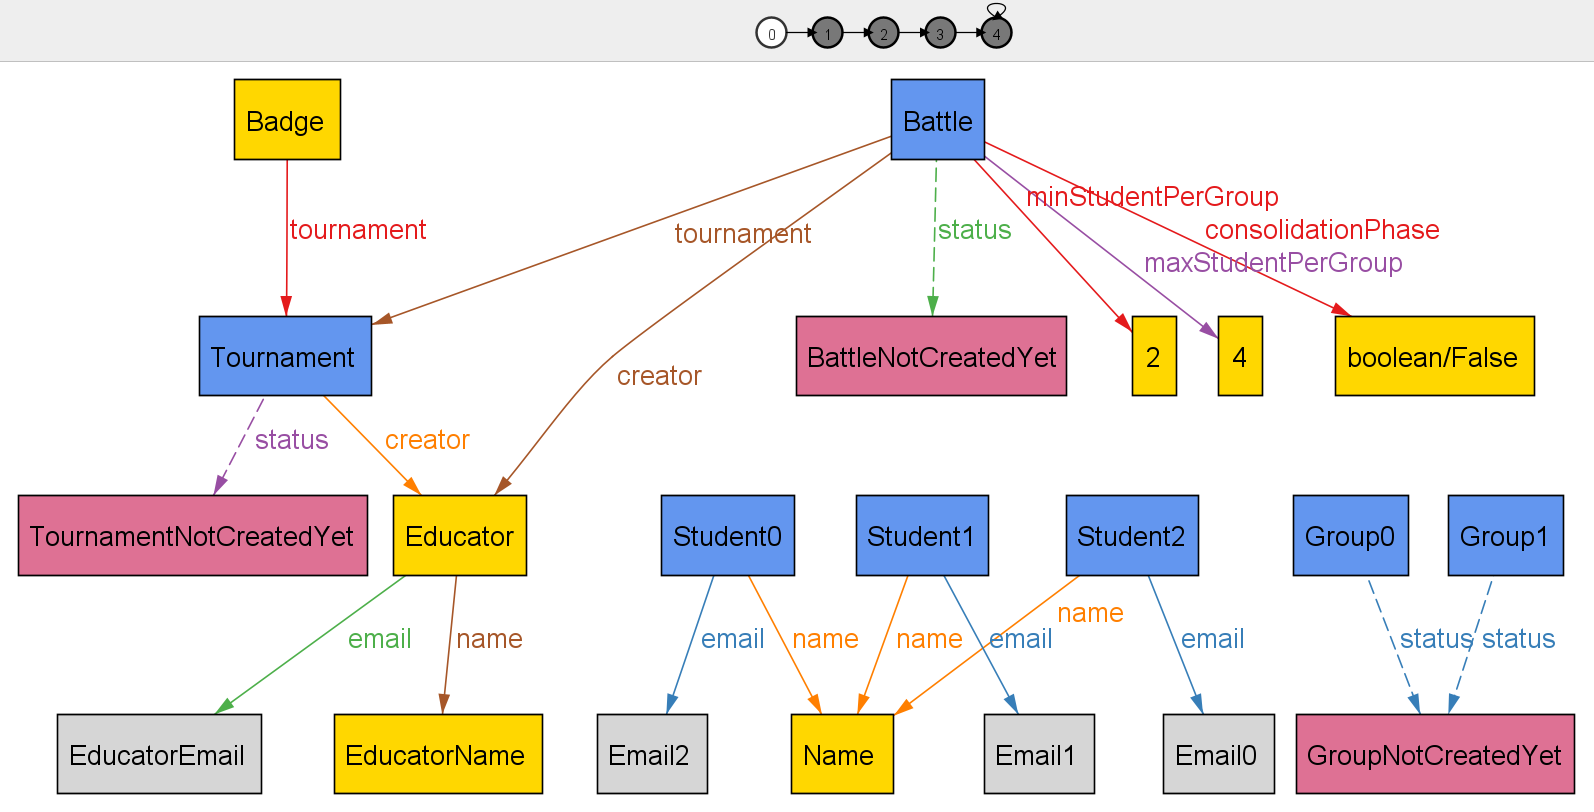
\includegraphics[scale=0.45]{Images/AlloyStep0.png}
    \caption{Initial state of the model}
    \label{fig:step0}
\end{figure}

In Figure \ref{fig:step0} we can see the initial state of the model. Starting with the time-independent constraints, we see that all the students have unique Emails (while having the same Name is allowed) and the Battle has coherent constraints: the number of students per group must be between two and four.

Concerning time-dependent constraints, we can see that the tournament, the battle and the two groups are in the \textit{NotCreatedYet} states, and no registrations by students or groups have been made so far.

\newpage

\paragraph{First step: tournament creation}
\textbf{ }\\

\begin{figure}[h]
    \centering
    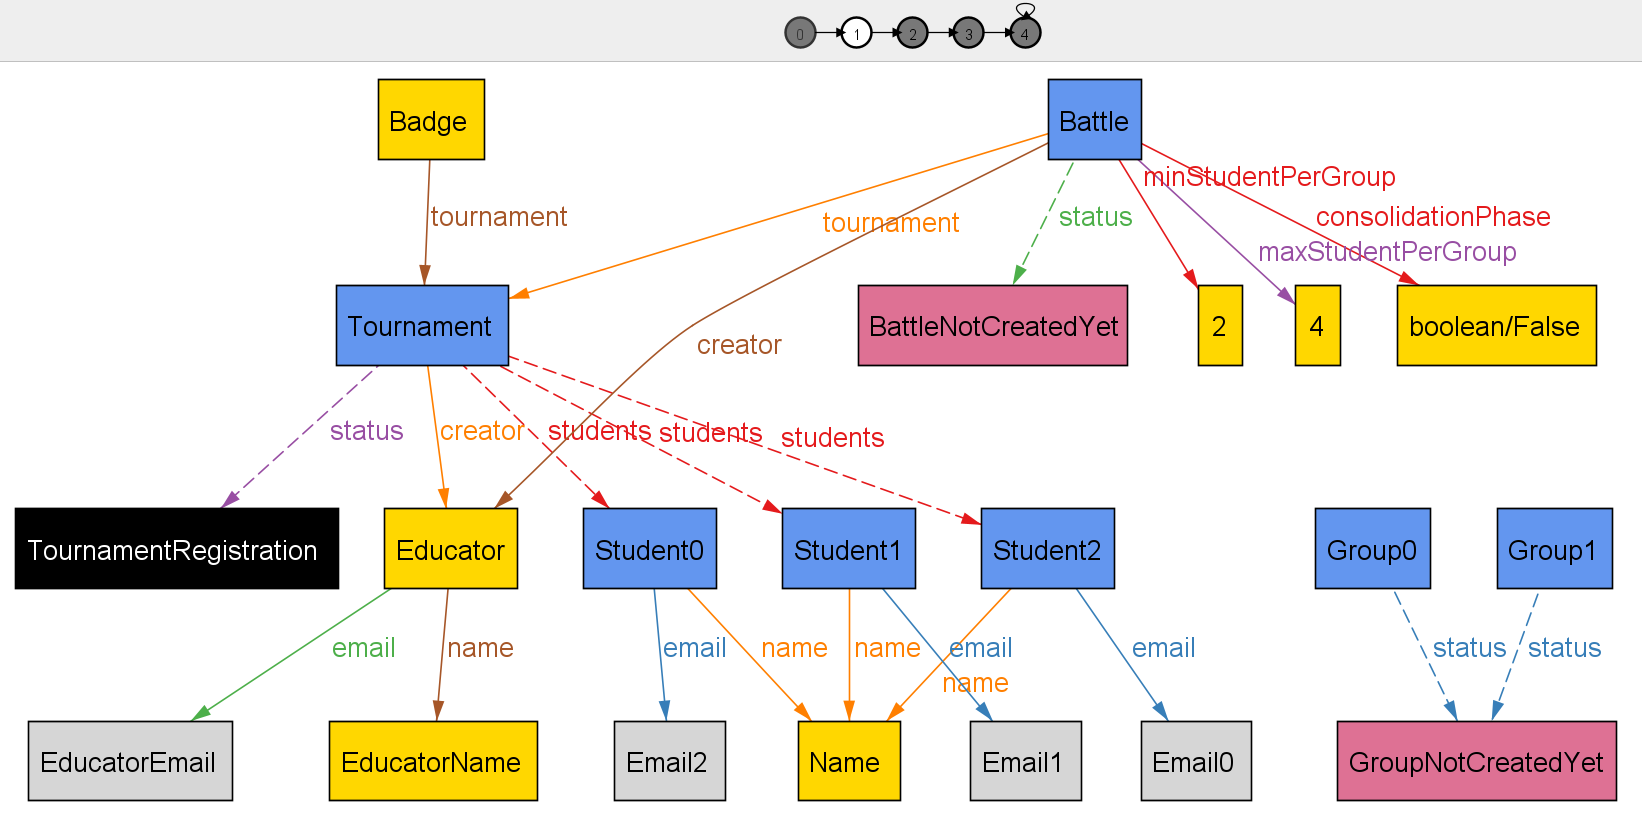
\includegraphics[scale=0.45]{Images/AlloyStep1.png}
    \caption{Model after 1 step}
    \label{fig:step1}
\end{figure}

In Figure \ref{fig:step1} we can see how the system evolves after one step: the tournament has been created and the status of the tournament is now \textit{TournamentRegistration}. As shown by the red dashed lines, the three students subscribed to the tournament. We can see how, since the tournament has not started yet, no battle has been created in the context of this tournament, and no group has been formed yet.

\newpage

\paragraph{Second step: battle creation}
\textbf{ }\\

\begin{figure}[h]
    \centering
    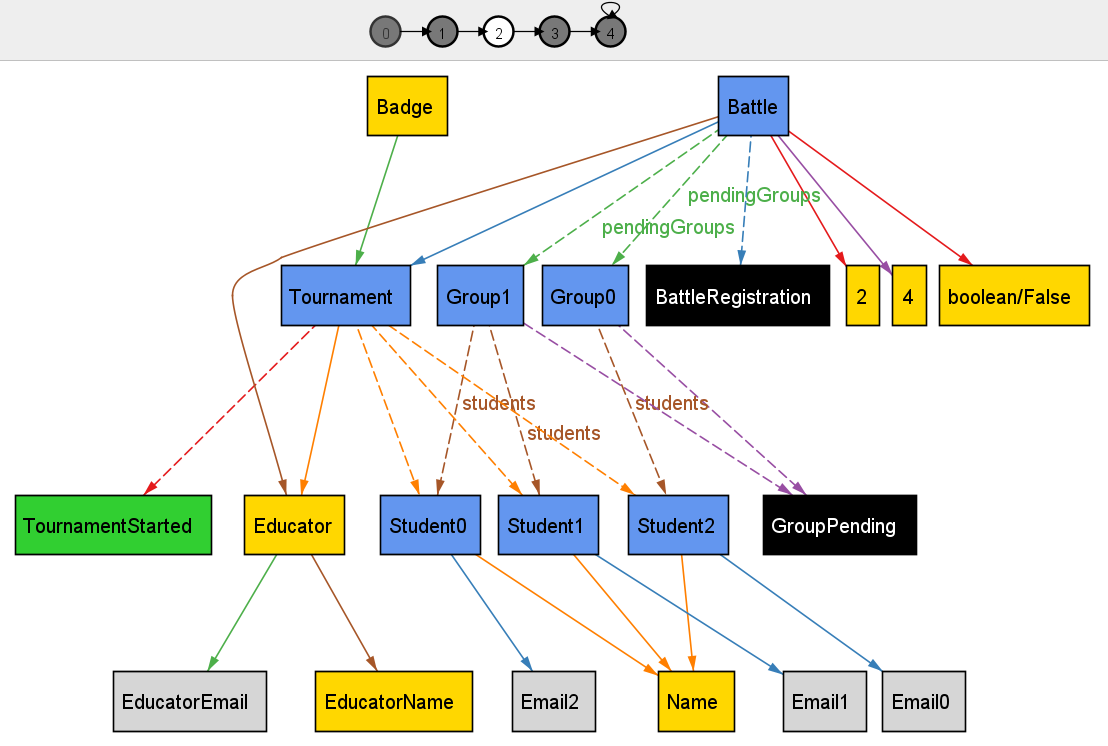
\includegraphics[scale=0.65]{Images/AlloyStep2.png}
    \caption{Model after 2 steps}
    \label{fig:step2}
\end{figure}

In Figure \ref{fig:step2} we can see how the system has evolved after the second step: the tournament has officially started. The Battle has been created and its state is \textit{Registration}. Two groups enlisted for the Code Kata Battle: one group is formed by Student 0 and 1, the other is formed by Student 2 alone. The state of the two groups is \textit{Pending} and they are in the list of \textit{pendingGroups} of the battle.

\newpage

\paragraph{Third step: group validation and start of the battle}
\textbf{ }\\

\begin{figure}[h]
    \centering
    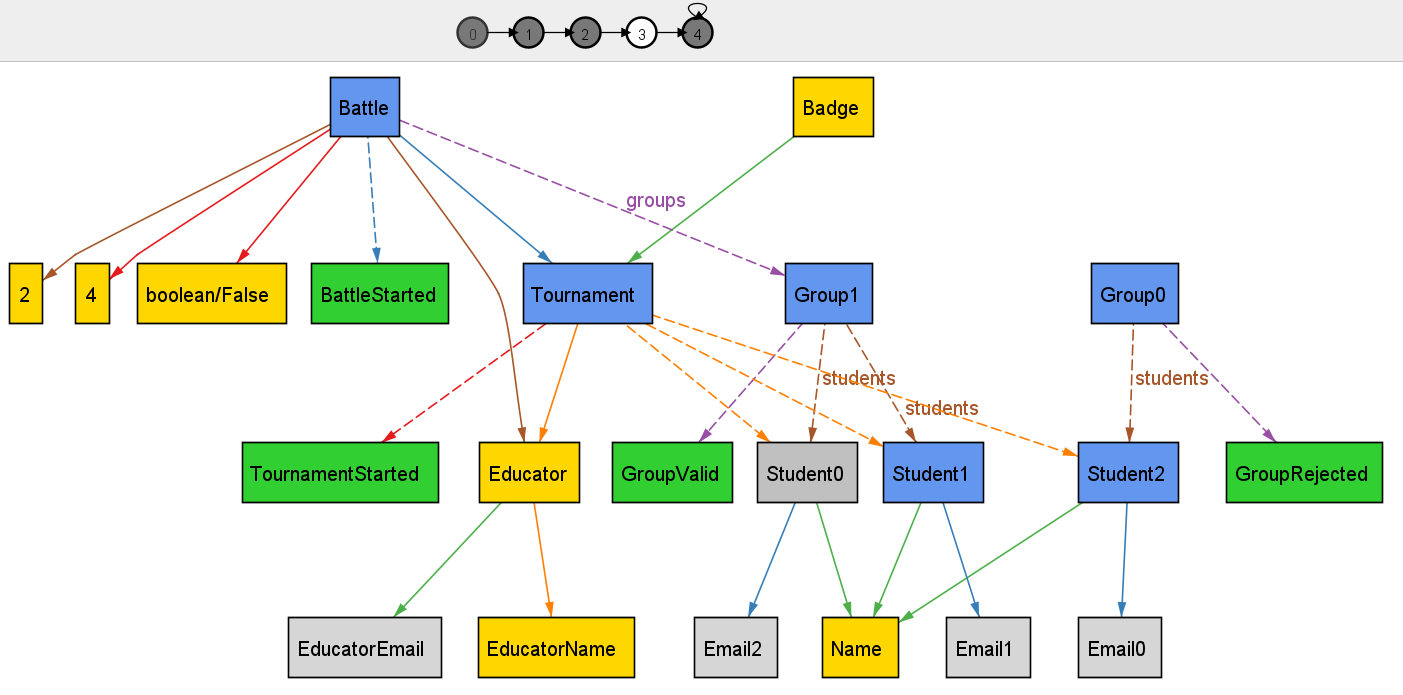
\includegraphics[scale=0.53]{Images/AlloyStep3.png}
    \caption{Model after 3 steps}
    \label{fig:step3}
\end{figure}

In Figure \ref{fig:step3} we can see how the system has evolved after the third step: the Battle has started. Since Group 0 had only one student it has been rejected (the minimum number of students per group in this battle is two), while Group 1 has been validated and inserted in the list of \textit{groups} of the battle. Since the Battle has not finished yet, the Tournament is still in the \textit{TournamentStarted} state.

\newpage

\paragraph{Fourth step: tournament closure and badge awarding}
\textbf{ }\\

\begin{figure}[h]
    \centering
    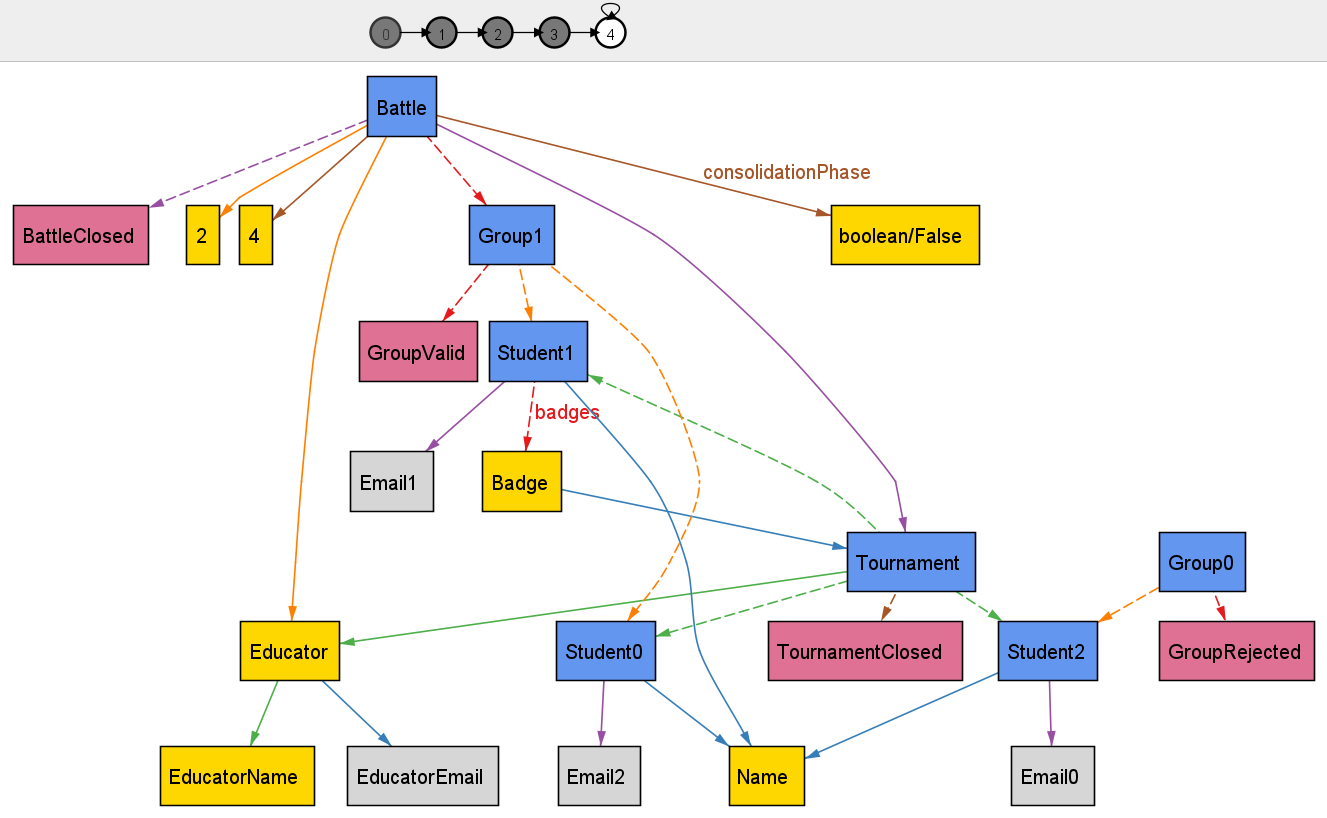
\includegraphics[scale=0.53]{Images/AlloyStep4.png}
    \caption{Model after 4 steps}
    \label{fig:step4}
\end{figure}

In Figure \ref{fig:step3} we can see how the system has evolved after the fourth and last step. Since the \textit{consolidationPhase} parameter of the Battle is false, the Battle has closed without the need of manual evaluation by the educator. The tournament has closed too, and the badge associated with the tournament has been awarded to Student 1. This is the last step of the execution: all the time-steps presented in this section are coherent with the specification of the system and its requirements.